\documentclass[a4paper,12pt]{article}

\usepackage[T1]{fontenc}
\usepackage[active]{srcltx}
\usepackage[english]{babel}
\usepackage[numbers]{natbib}
\usepackage[utf8]{inputenc}
\usepackage{amsmath}
\usepackage{amssymb}
\usepackage{fullpage}
\usepackage{graphicx}
\usepackage{listings}
\usepackage{parskip}
\usepackage{srcltx}
\usepackage{subfigure}
\usepackage{url}

\urlstyle{same}

\newcommand{\m}[1]{\boldsymbol{#1}}
\renewcommand{\*}[0]{\cdot}
\renewcommand{\Pr}[1]{\mathbf{Pr}[#1]}
\renewcommand{\v}[1]{\vec{#1}}
\newcommand{\trans}[2][eng.]{(#1 \emph{#2})}

\title{
    {\sc DD2380 Artificial intelligence} \\
    Project report from group PIMP
}
\author{
    \small
    Linus Wallgren \\ 880213 \and
    Joel Bohman \\ 881117 \and
    Samuel Lidén Borell \\ 881230 \and
    Joel Pettersson \\ 880519 
}
\date{\today}

\begin{document}
\maketitle

\begin{figure}[h!]
    \begin{center}
        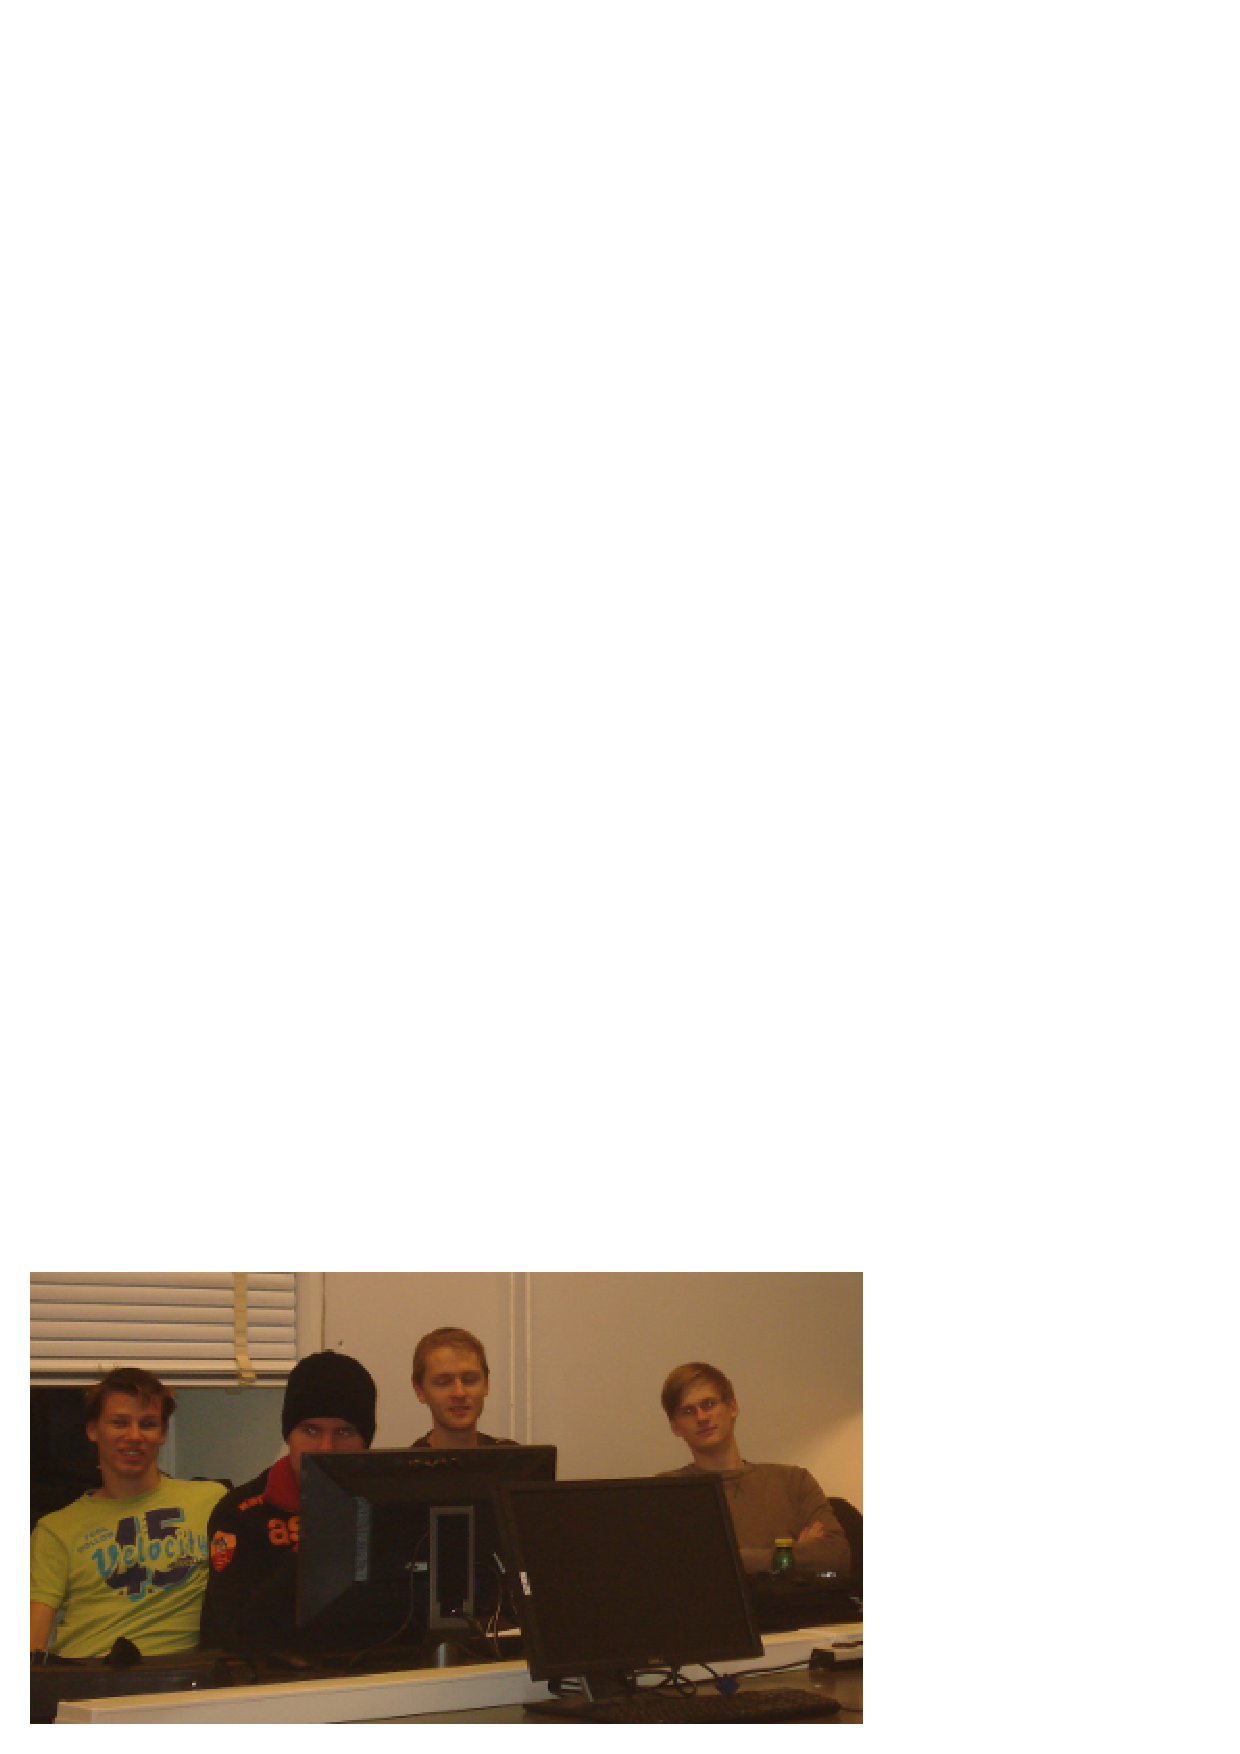
\includegraphics{figures/gruppbild}
    \end{center}
\end{figure}

\thispagestyle{empty}
\newpage
\begin{abstract}
    In this report we present our work with a solver for the puzzle game
    Sokoban. Boards in this game can have a very large number of possible
    states and is even PSPACE-complete, which implies that it is also NP-hard.
    We have implemented two solvers, that search forward and backward, and a
    third solver that performs significantly better using a combined,
    bidirectional search. We have used existing techniques such as
    transposition tables with Zobrist hashing, as well as a few novel ones.
\end{abstract}
\thispagestyle{empty}
\newpage
\setcounter{page}{1}


\part*{Introduction and background}

% - Some kind of introduction and one or two paragraphs about current solvers.
% - Short introduction to the problem and a description of the relationship to
%   the course material. also present what you think are your biggest
%   contributions so that this is clear. be sure to credit anyone that you got
%   help/code from

Sokoban is a puzzle created in 1981 by Hiroyuki Imabayashi. Sokoban is a
difficult puzzle and it has been proven that it is
PSPACE-complete~\cite{culberson1997}, which is a superset of NP. Current
solvers use techniques such as iterative deepening search (IDS), depth-first
search (DFS), breadth-first search (BFS), A* and combination of them to
traverse the search tree. Sokoban has a large branching factor which result in
a large search tree. To be able to traverse the search tree in any reasonable
time, pruning techniques and heuristics are necessary. Humans can solve
Sokoban puzzles by advanced heuristics that becomes natural to us after playing
the game for a while.


\section{Problem statement}

% a clear formalization of the problem using course material: which methods, how and why

Our task is to implement a program that is able to solve as many Sokoban levels
as possible. We have received test data that contains 136 levels to test our
solver against. However, we are not supposed to specialize our solver(s) for
this set of levels.


\part*{Theory and method}

% Explain the solutions we tried, answer why, how and what?
% A summary of your design approach and implementation

Sokoban can be solved by many different methods, as it is NP-hard and
PSPACE-complete it has not been proven that there exists an optimal solution,
but there are ways to prune the search tree and different kinds of heuristics
that can be used to find a solution faster. Our focus has been on pruning
techniques to reduce the size of the search tree, with heuristics for choosing
the search depth and solver. Our work resulted in three different solvers ---
IDSPusher, IDSPuller and a Bidirectional search combining them both.


\section{Solvers}

We chose to use iterative deepening search, also called IDS, when
implementing the solvers. The reason we chose IDS over breadth-first search,
BFS, was simple, memory consumption. A normal BFS would need to store every
board state it intends to visit in a queue, which would require large memory
footprint. Our original assumption was that depth-first search, DFS, would go
down too deep into the tree and possibly go past solutions, which was the
reason we originally chose IDS. IDS is simply a DFS that only goes down to a
certain level in the search tree, if we find the solution we are done, otherwise we
increase the depth and try again.

When we began to implement the bidirectional search we found that IDS was
perfect, as we could simply let the solvers take turn going deeper.

\subsection{IDSPusher}

To push the boxes around is the most natural solution, as it is how the game
actually works. The basic idea was a brute-force approach that mimicked the
human way to solve Sokoban puzzles. The naive implementation of a pusher is
simple and easy to understand, however it is not particularly effective.
Because of this we implemented a couple of pruning techniques, like tunnel
detection and deadlock detection, which will be described later.

\subsection{IDSPuller}

Puller is our name for a method in which we reverse the goal and box positions.
Instead of trying to push boxes from their start positions to their goal we try
to pull boxes from the goals to their start positions. The advantage of this
approach is that no so called freeze deadlocks can occur~\cite{takes2007},
which reduces the number of useless state. This works because freeze deadlocks
occur when a box gets blocked by other boxes, and this can not happen when
pulling boxes because the player must be able to reach the square where the box
is to be pulled to. It is still possible however to move a box such that some
boxes can no longer be reached.


\subsection{Bidirectional search using IDSPusher and IDSPuller}

Bidirectional search is a powerful way to reduce the search tree a lot
search~\cite{russell2009}. Instead of letting one solver go all the way we let
two solvers take turn to solve the board from both ends. As the size of the
search tree is exponential there is a lot to gain from this approach. Let us
look at an example.

In a complete binary tree, there are $2^n$ nodes on the level at depth $n$.
Thus, the total number of nodes is $2^n + 2^{(n-1)} + \ldots + 2^0$. Thinking
of this as a binary number we see that $2^n > 2^{(n-1)} + \ldots + 2^0$, e.g.
$1000_2 = 8_{10} > 0111_2 = 7_{10}$. This implies that more than half of our
nodes are in the lowest level. When we use bidirectional search we only need to
search to half the depth --- two times. This means the number of nodes in the
lowest level will be $2^{(n/2)}$ for each one of the two solvers, which is much
less than the $2^n$ nodes required originally.

In a Sokoban problem the branch factor will typically be much higher than two
because there are often at least a couple of boxes that can be pushed from four
sides in the worst case (if there are no walls or other boxes at the sides).
That makes the bidirectional solver even more efficient for this kind of
search, even though pruning techniques may reduce the average branch factor.



\section{Pruning techniques}

\subsection{Repeated states}

One of the probably most important pruning strategy is to check for repeated
states. We might arrive at a state following different paths in the search tree,
and exploring a node is only necessary to do once. That is, if we reach a state
that we recognize, it is time to stop following that road. In order not to be
required to store the whole board in a transposition table for repeated states
checking, we have chosen to use a hashing algorithm called Zobrist keys. In
addition to reducing memory usage, this type of hashing also allows constant
time comparison of boards.


\subsubsection{Zobrist keys}

Zobrist keys~\cite{wiki:zobrist} is a hash function that seems to work quite well for games that has
perfect information\footnote{Every participant in the game knows all the moves}.
Sokoban is obviously such a game, which was the reason for us trying it out. The
hashing algorithm makes heavy use of the XOR operation and its property that
given two bitstrings $x$ and $y$, the result of $(x \oplus y) \oplus y$ equals
$x$.

We implemented it by generating a random number for every possible state ---
\emph{empty} or \emph{box} --- of every cell on the board, which are stored in a
three-dimensional array. In order to calculate the hash of a board, one must
start with an empty hash key and iterate over every cell on the board and
XOR in the corresponding random number for that cell and state . ``Now wait'',
you say, ``this requires $n^2$ operations''. And yes, that is true, however, the
next time we make changes to boxes on the board, we simply XOR out the box that
is being moved from its previous position and XOR it in to the new position.
That way, we have created a new hash key for an arbitrary box movement by
performing only two XOR operations, which only requires 2 operations.

``But hey'', you object, ``you have to take the player position in
consideration too''. And yes, that is also true. The naive solution would
simply be to let a cell have a state where the player is present, in addition
to the states \emph{empty} and \emph{box}. However, that would cause many
equivalent states to generate different hashes, like those in
Figure~\ref{fig:equalStatesDifferentHash}. For that reason, we instead keep
track of the top leftmost position that the player may reach without moving any
boxes and XOR:ing the hash with that position (which is actually also hashed).

\begin{figure}[h!]
    \begin{center}
        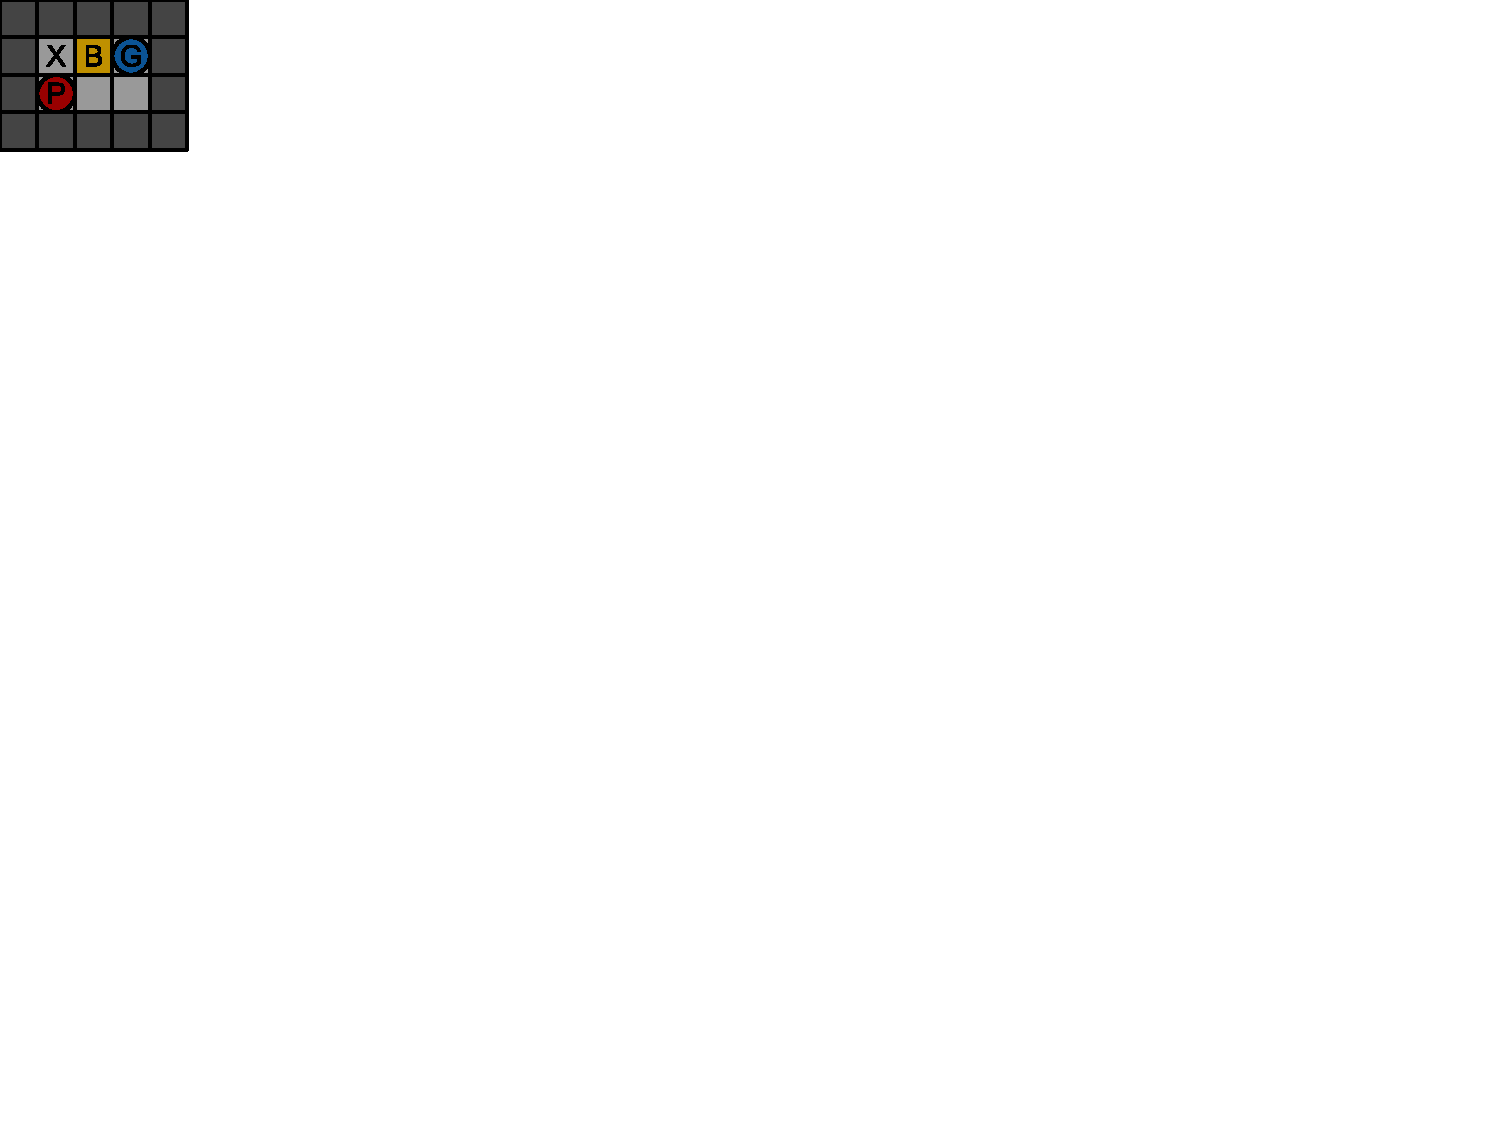
\includegraphics{figures/equalState1}
        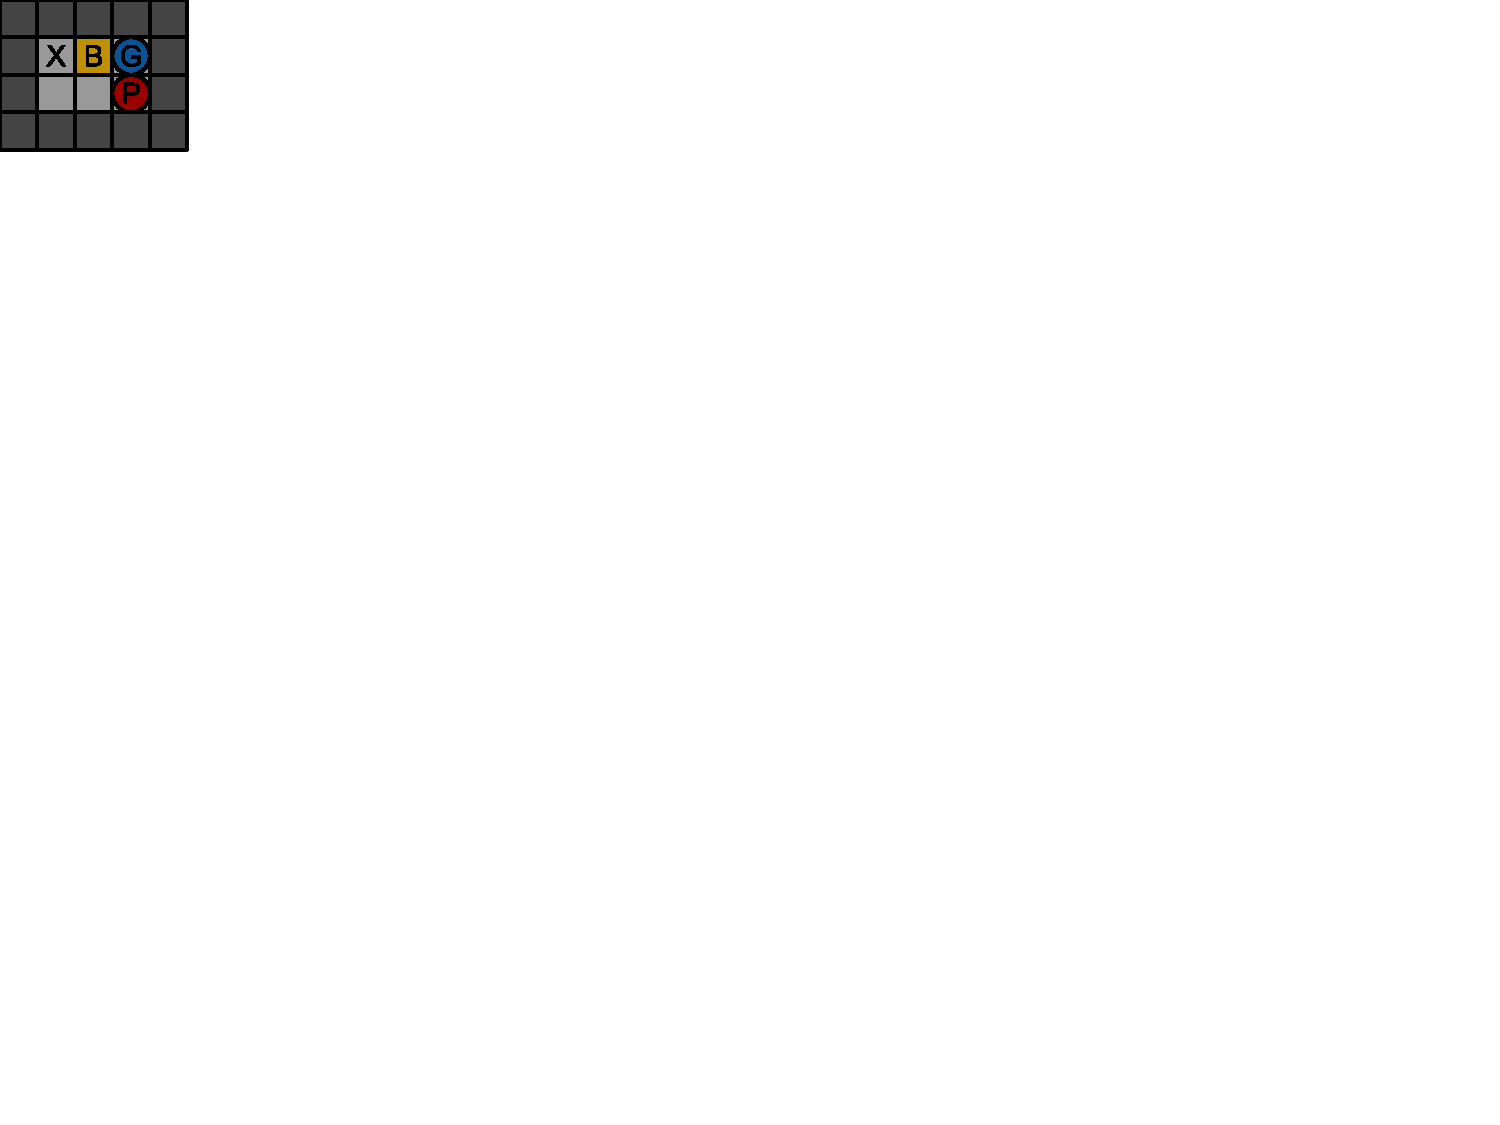
\includegraphics{figures/equalState2}
    \end{center}
    \caption{Notice how the two boards are equivalent, since the player may move
    between the two player positions without moving any boxes. This is the same
    as saying that the top leftmost position that the player can reach in both
    states is the same.}
    \label{fig:equalStatesDifferentHash}
\end{figure}

The beauty of Zobrist keys is that it, as mentioned above, only requires
constant time for each box move in the board, and also is reversible in some
sense. This turned out later to be very useful, when implementing the
bidirectional search solver. Thanks to the properties of Zobrist keys and only a
little additional information in every state (which box was pushed in what
direction and the player position), we are able to calculate the hash for the
next state, and thereby follow the other solver's path all the way into the goal
state.


\subsection{Deadlock}

Detecting deadlock is another important pruning technique. A deadlock is a
state where it is no longer possible to solve the puzzle. For example a deadlock
is achieved when a box move result in two or more boxes being stuck. Other boxes
can continue moving on the board until the search space is exhausted. When this
happens the solver need to backtrack to a previous state where the deadlock did
not occur. By finding this deadlock a large amount of nodes in the search tree
can be pruned.

\subsubsection{Dead squares deadlock}

A \emph{dead square} is a position from which a box can never be pushed into a
goal. These can be calculated statically for every board, as the only thing
required is the positions of the walls and these do not change during the game.
The most obvious case is a corner, from which a box can only be reached from two
directions but is blocked by a walls at the opposite sides. This is used as a
starting point in our dead square detection algorithm.

We extended the dead square detection further by starting from the previously
marked dead squares and checking if the squares to the right and below can only
be moved into this square or a later dead square on the same row or column,
respectively. In that case we mark the squares to the right and below as dead
squares. This algorithm is iterative and continues until no more changes can
be made.

\begin{figure}[h!]
    \begin{center}
        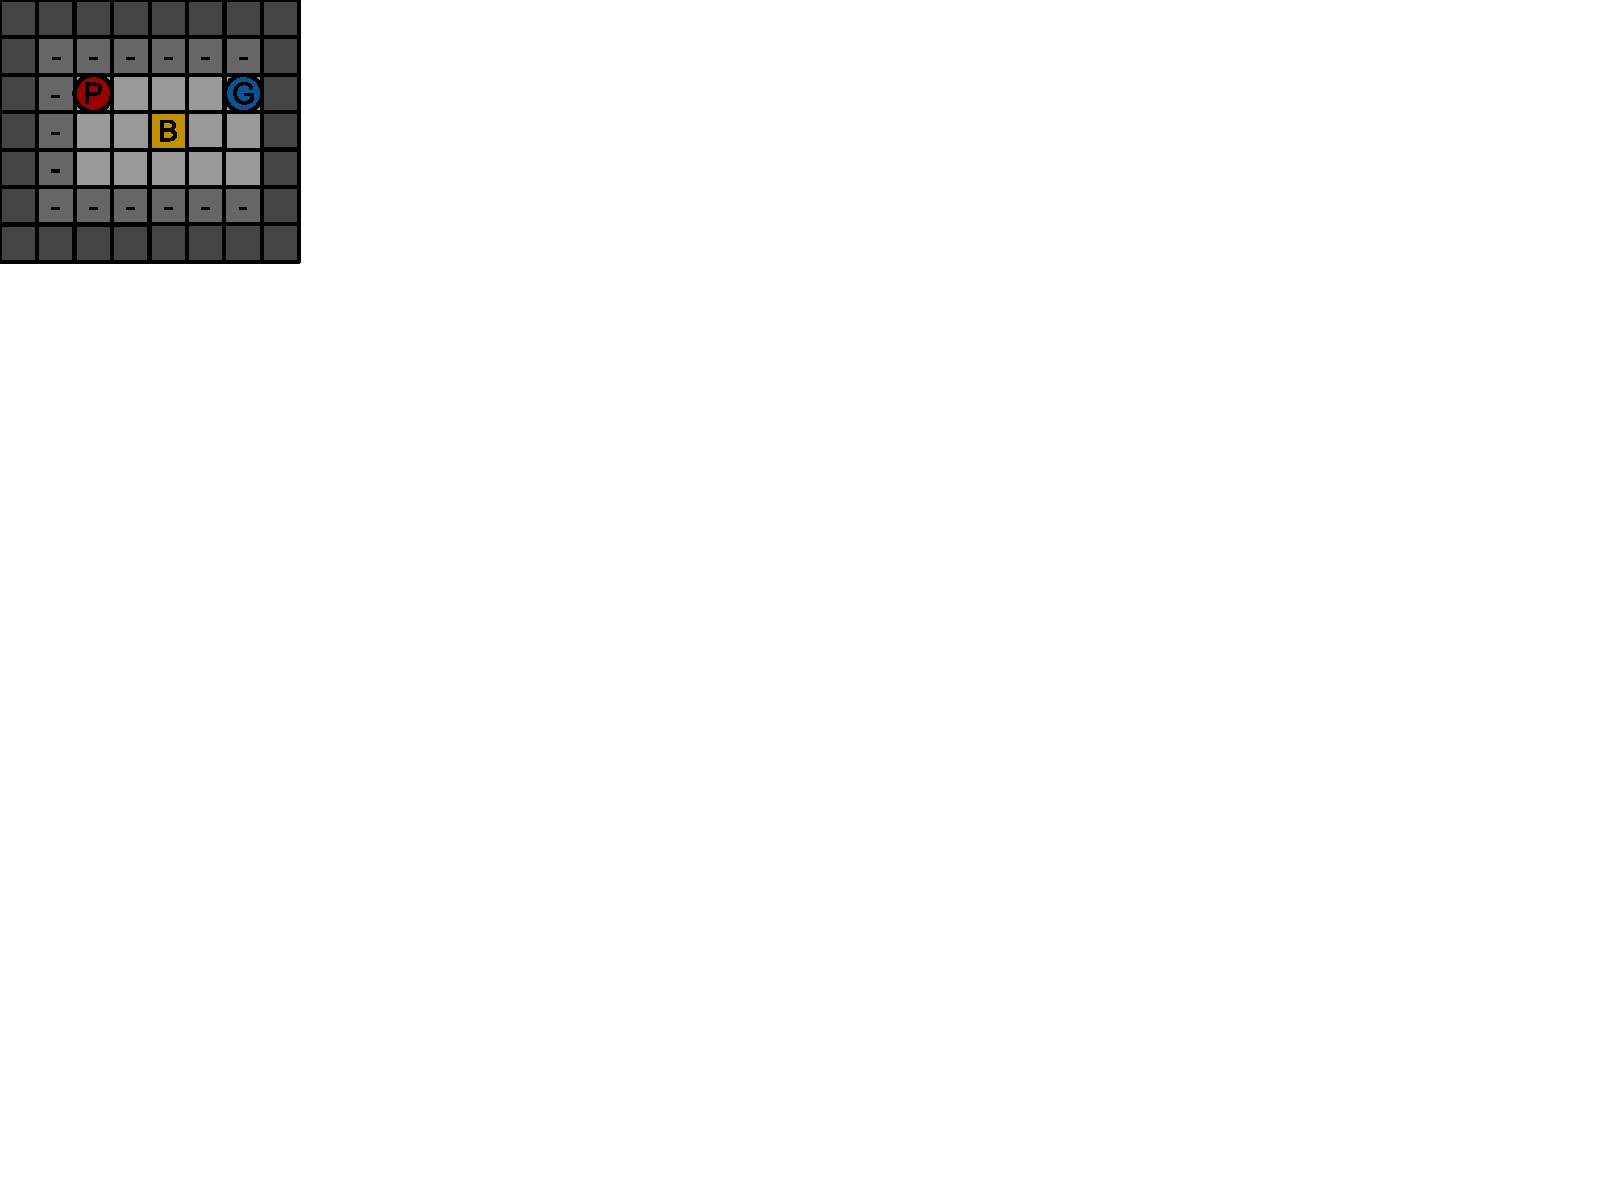
\includegraphics{figures/deadSquareDeadlock}
    \end{center}
    \caption{An example of a dead square deadlock marking. The dead squares are
    marked with a minus sign (-).}
    \label{fig:deadSquareDeadlock}
\end{figure}

\subsubsection{Freeze deadlock}

Another type of deadlock is a \emph{freeze deadlock}~\cite{sokobano:deadlocks}.
This occur when a box gets blocked by a wall, dead square or another box.
Because we care for other boxes this check must be recursive with a max
recursion depth of the amount of boxes in the map. The most simple freeze
deadlock is illustrated in Figure~\ref{fig:freezeDeadlock}, where the two boxes
is locked into their current position by each other and the wall above.

\begin{figure}[h!]
    \begin{center}
        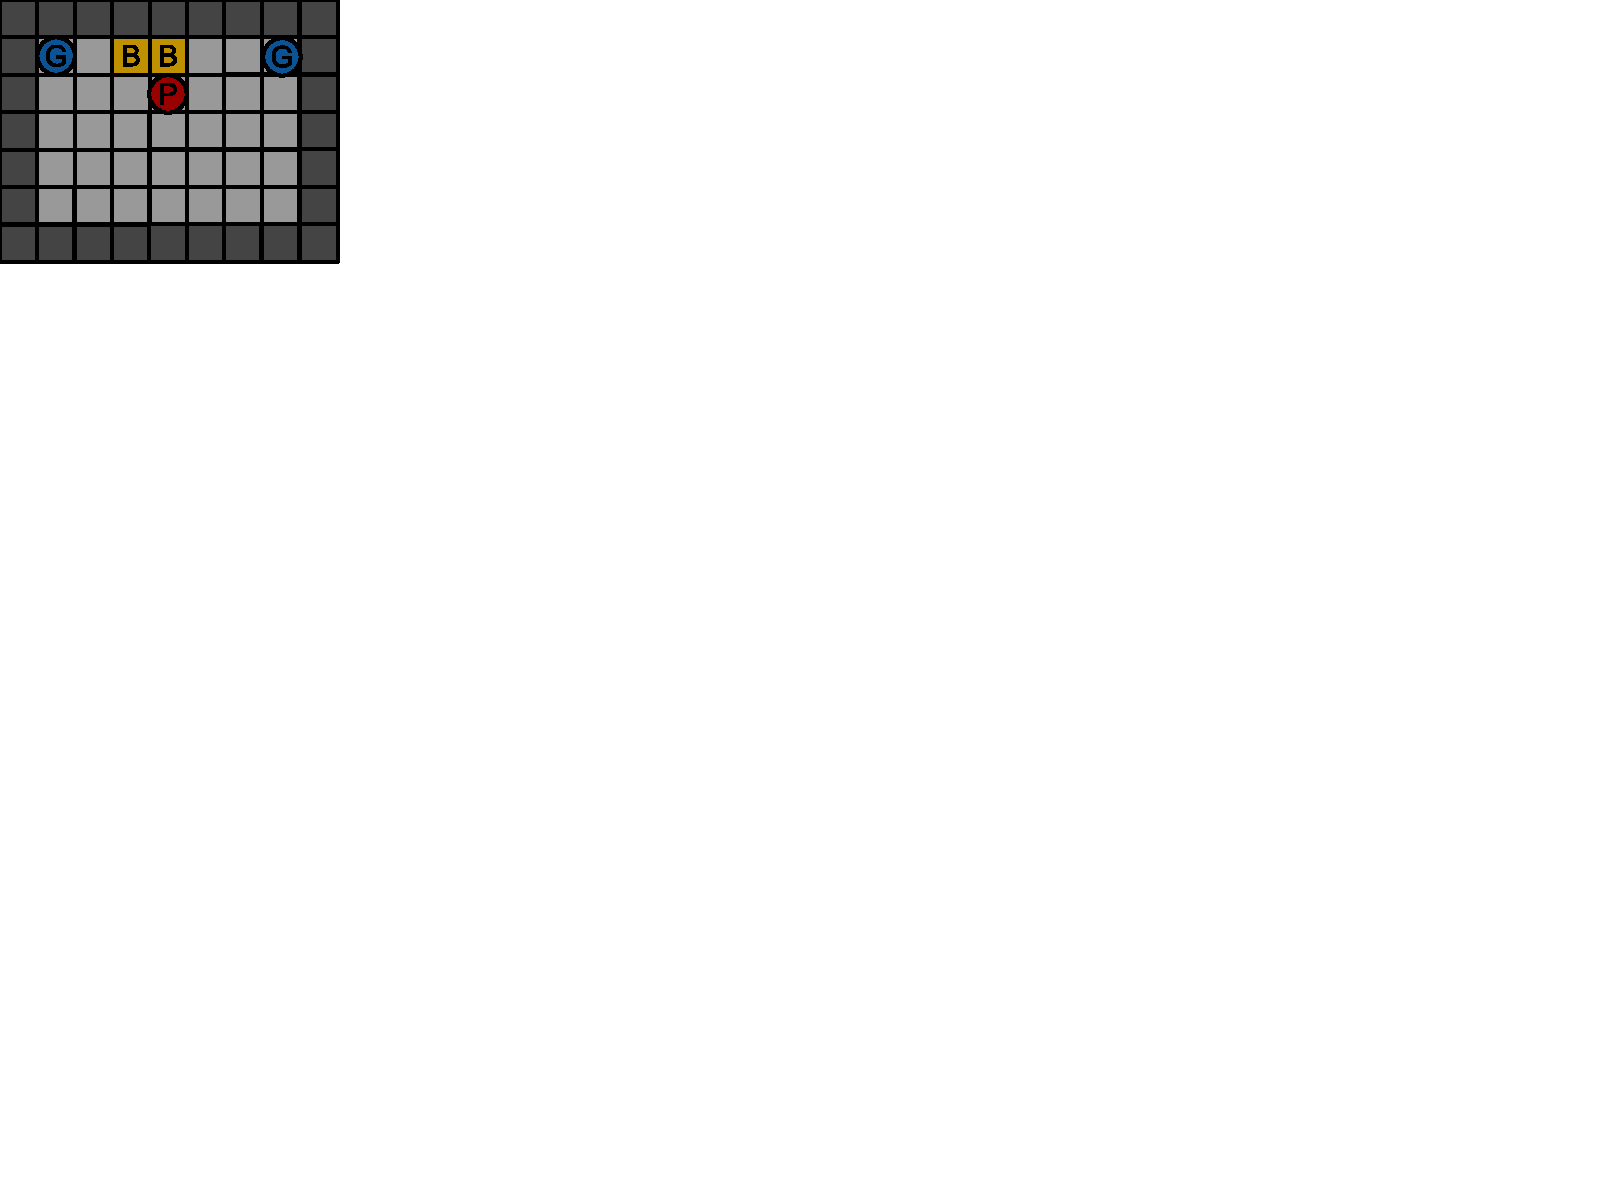
\includegraphics{figures/freezeDeadlock}
    \end{center}
    \caption{An example of a freeze deadlock.}
    \label{fig:freezeDeadlock}
\end{figure}


\subsection{No influence pushes --- tunnels}

A \emph{no influence push} is a push of a box that does not influence the board
but eventually have to happen~\cite{sokobano:noinfluence}. If such pushes can
be found and grouped together we can remove all those individual moves from the
search tree and decrease the size of it.

Tunnels is a type of no influence pushes and it is the only such strategy that
we have tried to implement. If a box is pushed inside a tunnel it makes no
difference to the boxes outside the tunnel how far the tunnel box is pushed
inside the tunnel. When we push a box inside a tunnel a new state is generated,
from this state we generate all successor states, that is we try to move all
the boxes on the board. The reason this is bad is because there is only one
thing we can do with the box inside the tunnel, so each push on another box is
done in vain, as we need to push on the box inside the tunnel sooner or  later.

In order to solve this problem we simply look at cells in a $2 \times 3$ square
around the box to see if it is a rotated or mirrored version of the states
illustrated in Figure~\ref{fig:tunnelPossibilities}. Each time we detect such a
state we can simply move the box one more step and begin again with checking if
this new box position is inside a tunnel as well.

\begin{figure}[h!]
    \begin{center}
        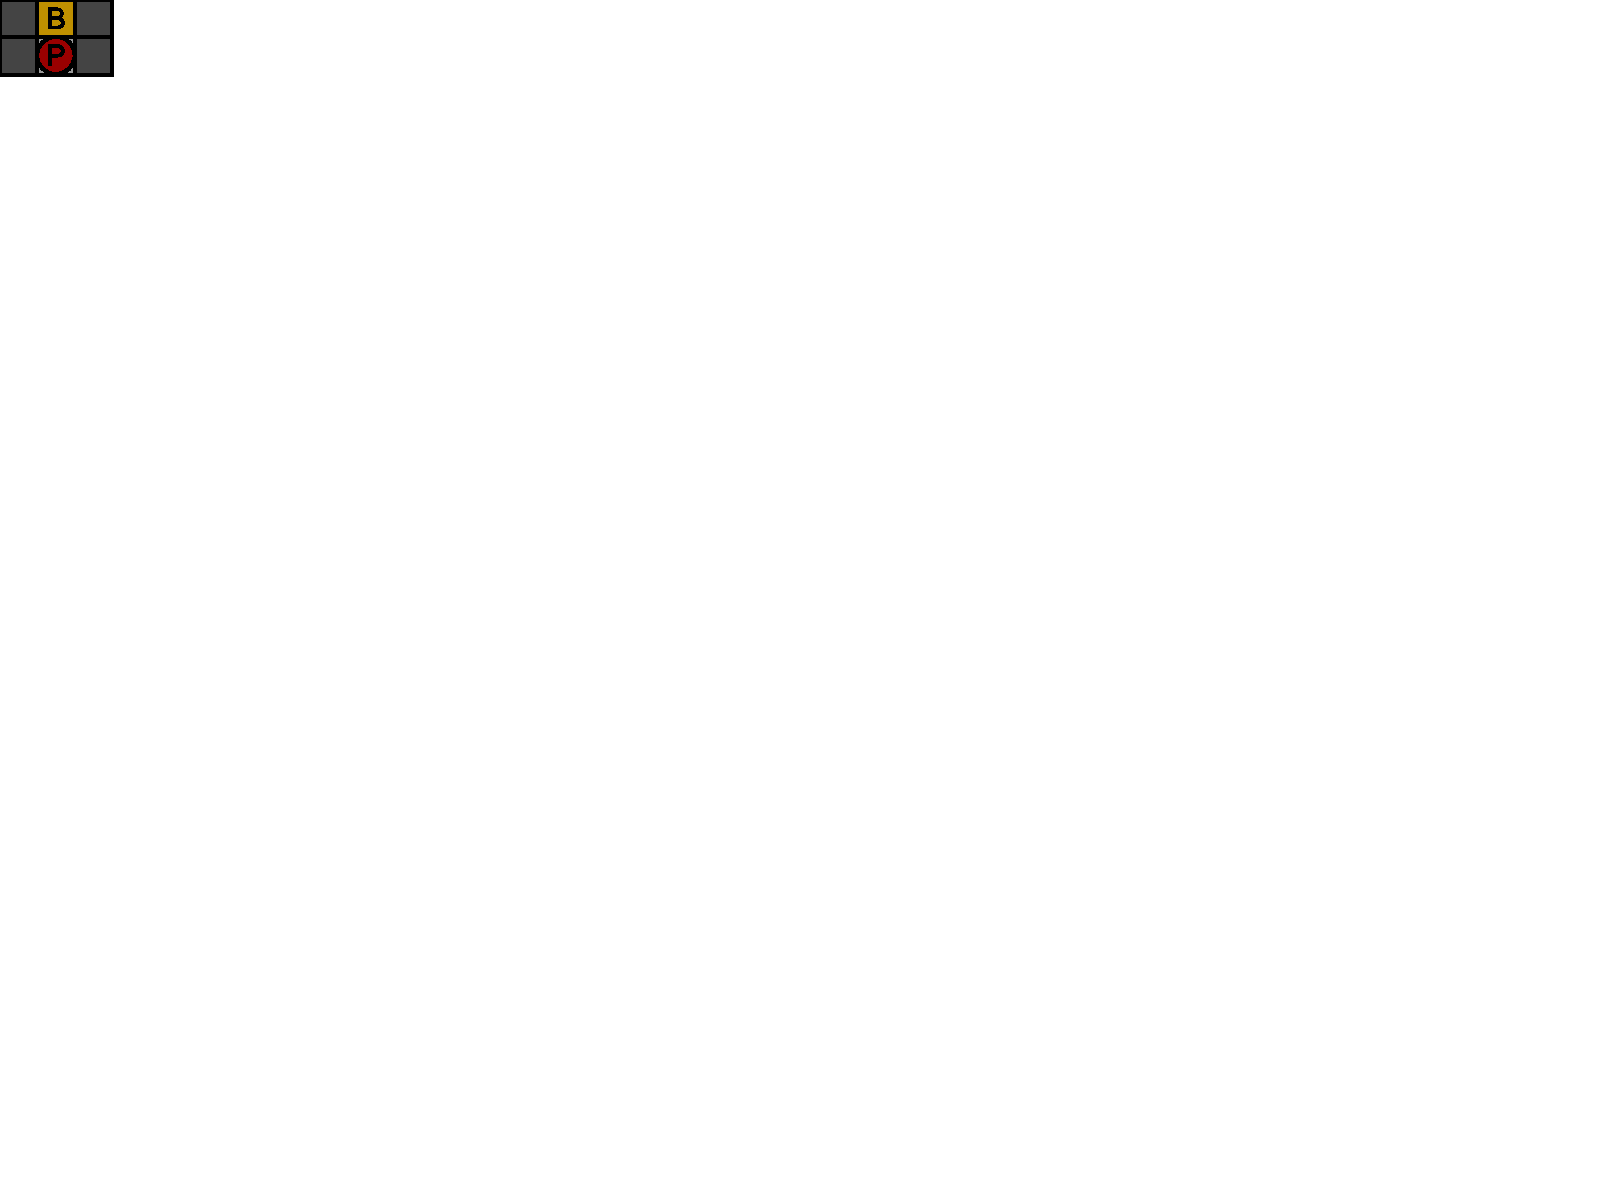
\includegraphics{figures/tunnelPossibilities1}
        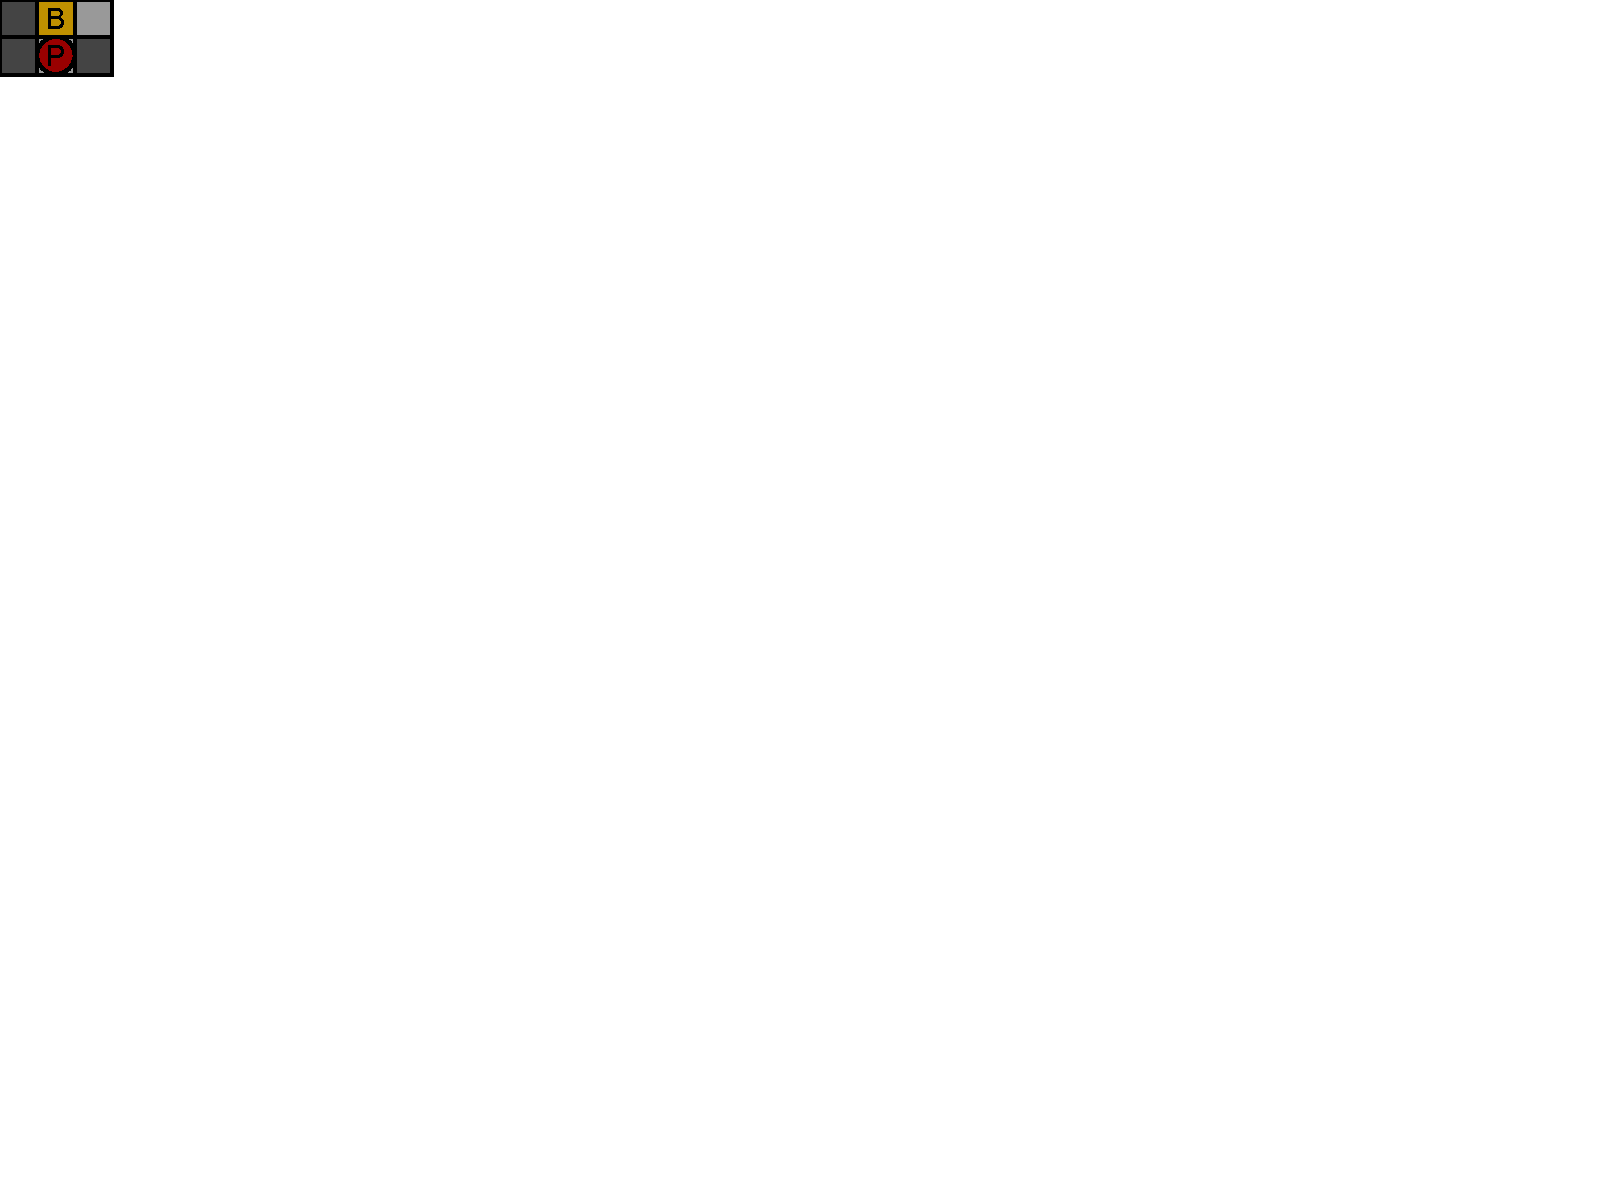
\includegraphics{figures/tunnelPossibilities2}
    \end{center}
    \caption{List of possible tunnel states. Must be mirrored and rotated to be
    comprehensive.}
    \label{fig:tunnelPossibilities}
\end{figure}


Figure~\ref{fig:insideTunnel} gives an example of what should be done inside a
tunnel. In the first state we need to expand all possible movements regarding
all boxes on the field. However in the second state illustrated we can be sure
that the correct movement is forward, as we just came from the only other
possible state when moving that particular box. This means that when we arrive
at a state that resembles the second state in Figure~\ref{fig:insideTunnel}, we
can directly push the box forward until we reach the third state.

\begin{figure}[h!]
    \begin{center}
        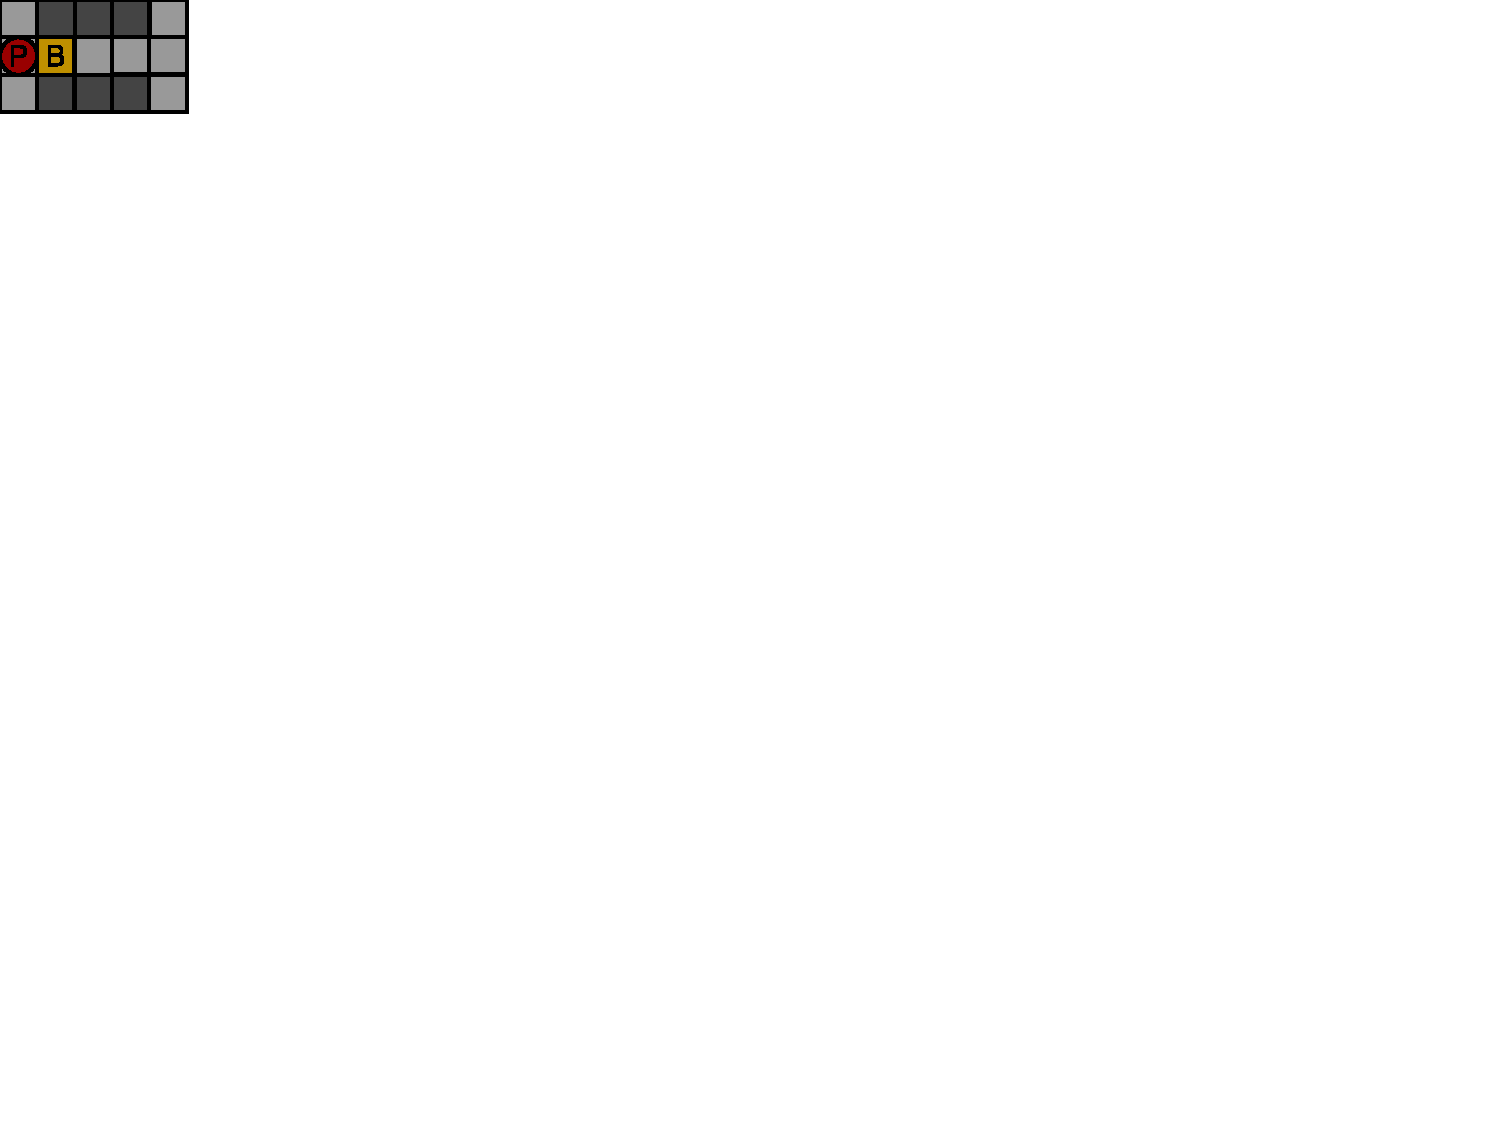
\includegraphics{figures/insideTunnel1}
        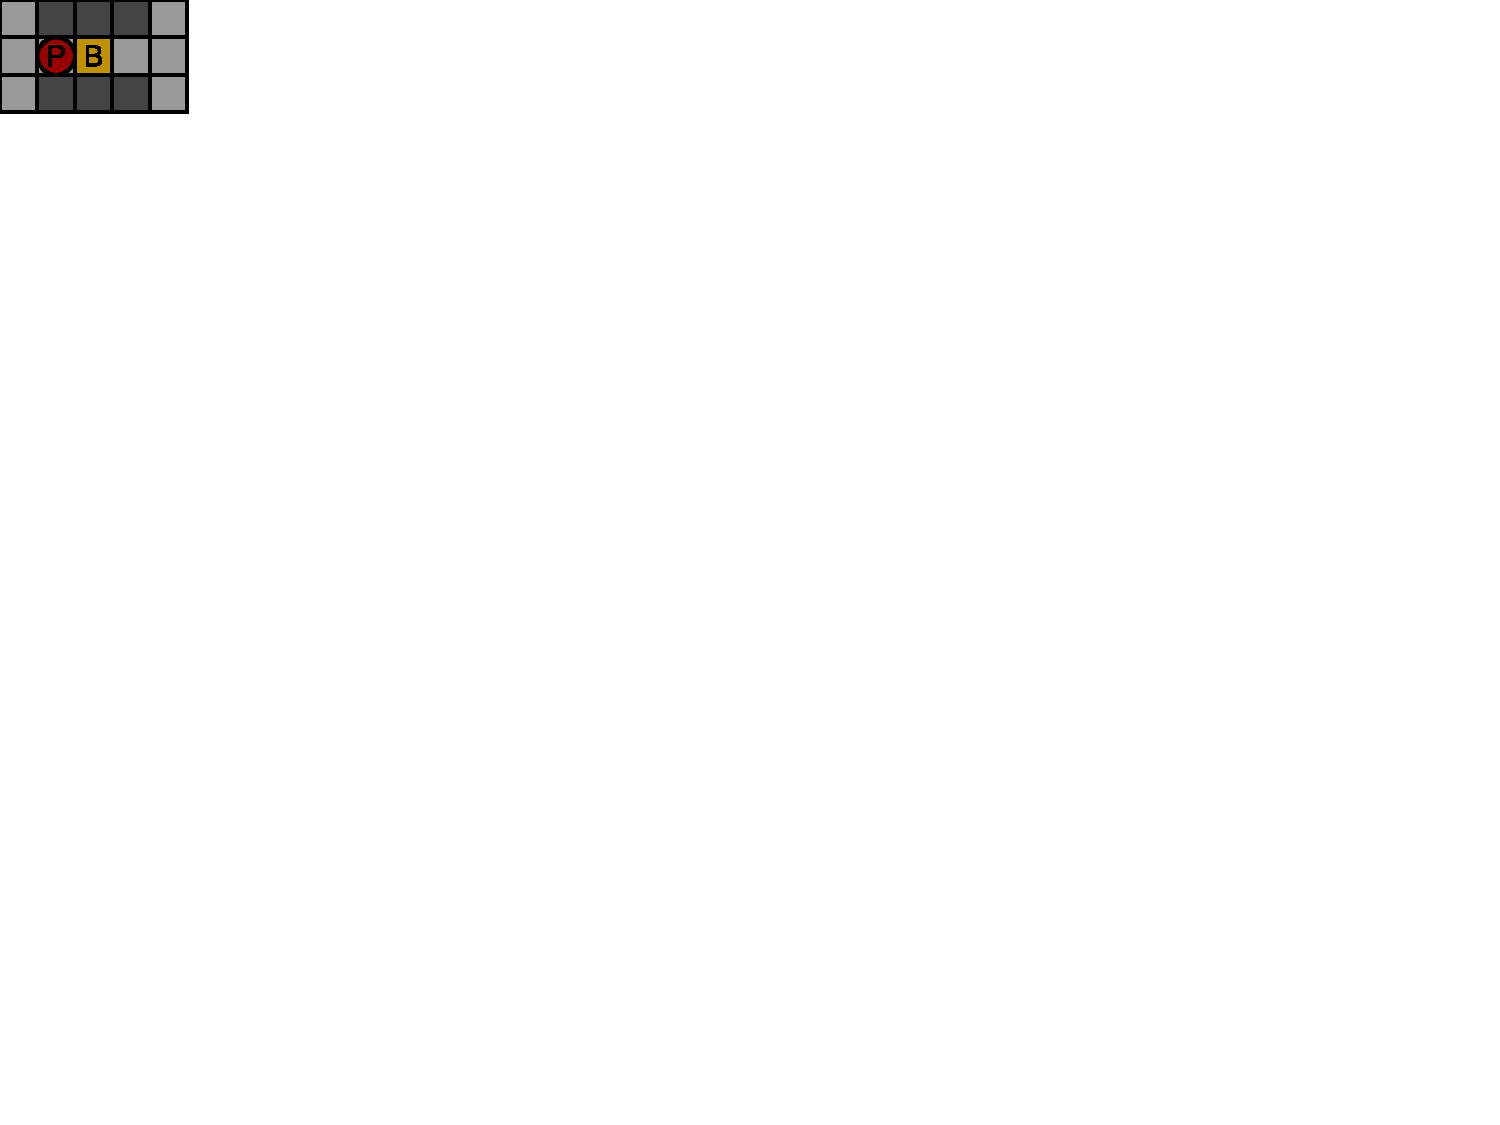
\includegraphics{figures/insideTunnel2}
        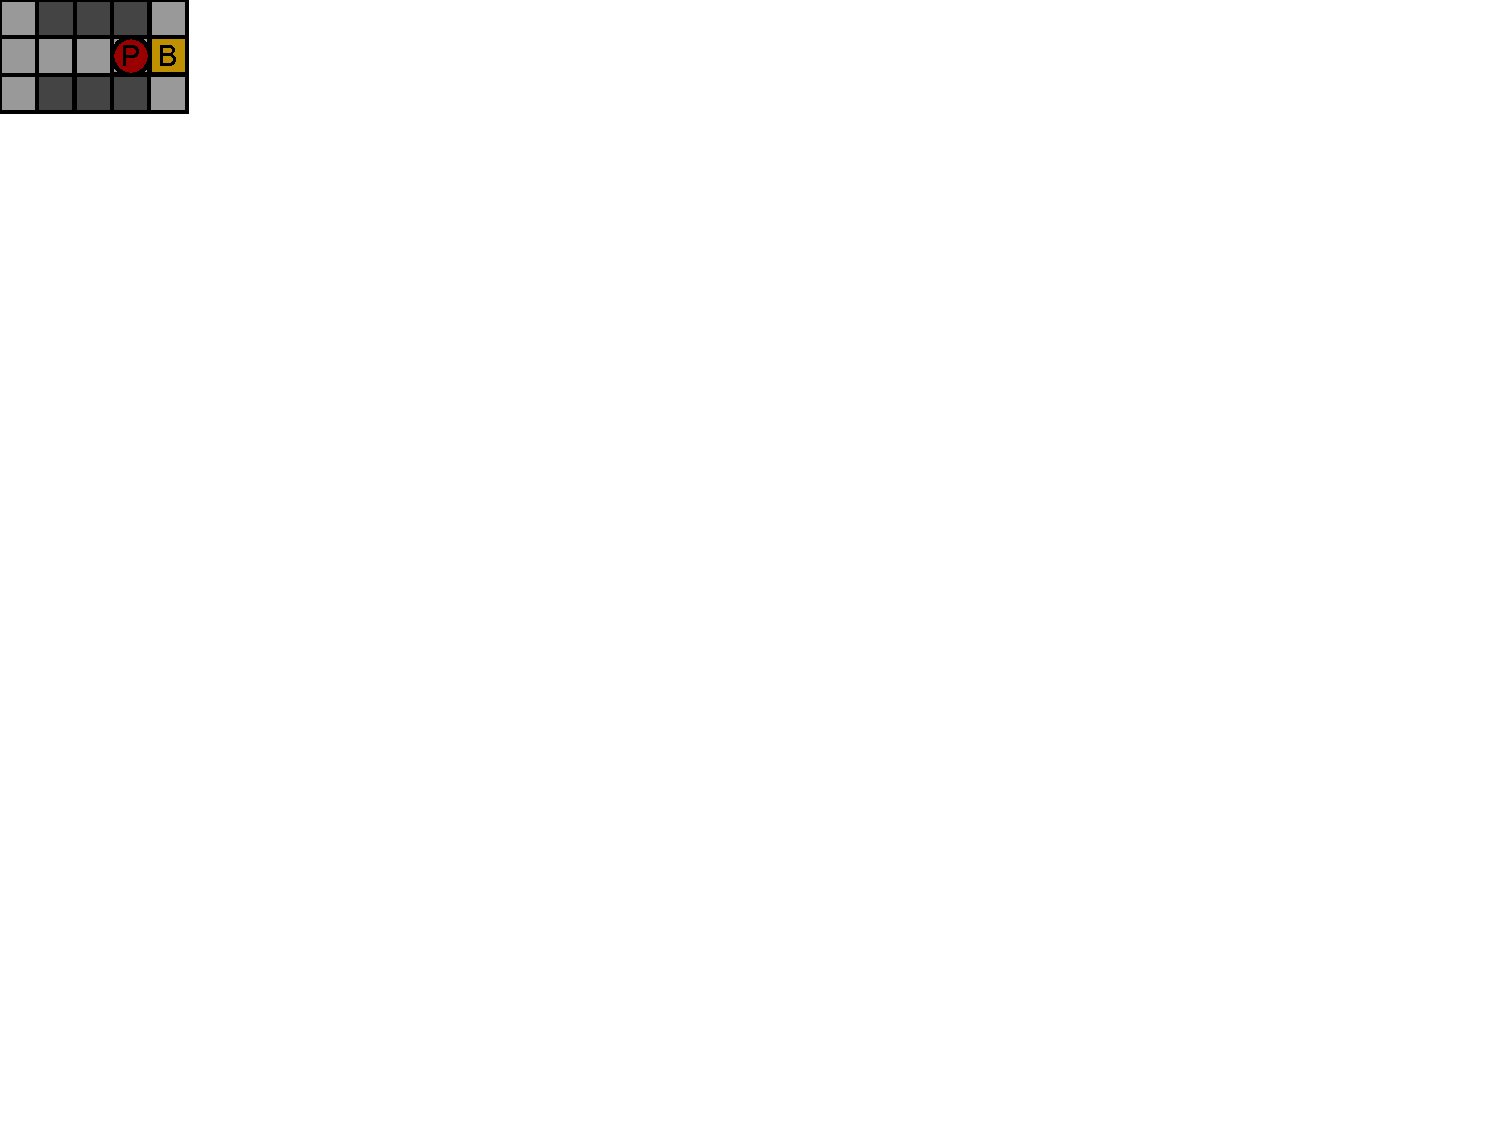
\includegraphics{figures/insideTunnel3}
    \end{center}
    \caption{Sequence of tunnel states.}
    \label{fig:insideTunnel}
\end{figure}

% TODO fixa 5a, 5b, 5c om möjligt
% subfigure isf


\section{Heuristics}

\subsection{Lower bound}

Before we start searching we use a greedy algorithm to calculate the minimum
distance in squares between the boxes and the goals, and use this value as the
search depth limit in the initial iteration of our IDS. This reduces the number
of iterations that have to be performed as we can be certain no solution will be
found above this depth. This is true in the bidirectional solver as well. As the
bidirectional solver consist of two separate solvers each of them only need to
go half the distance in order to meet in the middle, which is the reason we
choose to halve the lower bound for each solver in the bidirectional search.

\subsection{Adaptive deepening}

Similarly to the lower bound we use a heuristic to choose the search depth limit
for subsequent iterations. This is based on the number of leaf nodes, where we
look at the ratio between the current and the last iteration. In case of a
higher ratio, where the number of leaf nodes is constant or decreasing we make a
larger step. Again, this reduces the number of iterations needed to solve the
board.

\subsection{Choosing solver}

In our bidirectional solver we need to choose which direction to search from in
each iteration (from the start state and forward or from the goal state and
backward). We choose the solver with the minimum number of leaf nodes, because
we expect that solver to go deeper down the tree faster, as it probably has
fewer nodes to expand.

\part*{Results}

% Our result, how many did we solve? List run times, important and interesting data
% A thorough analysis of your experimental results

We successfully solved 111 of 136 of the problems listed in 60 seconds with our
bidirectional solver. Of these, 45 were solved in less than a second. The
remaining 25 problems could not be solved because the solver expanded to many
nodes in our search tree. The bidirectional solver was able to solve many more
boards than IDSPusher (71 boards) and IDSPuller (80 boards) individually (that
is, it solved almost 39 \% more than the puller). It should also be said that
the bidirectional solver not only solves more boards, but increases the speed
greatly of the boards it already solved.

When running the individual solvers (IDSPusher and IDSPuller), we saw that the
puller was able to solve a few more boards than the pusher. On the boards that
both could solve, puller was generally faster, and on a few boards it was as
much as 5 times faster. Because the two solvers were based on the same code and
had only minor differences, this suggests that the puller was indeed avoiding
more types of deadlocks.

Before we implemented the solvers using iterative depth-first search we tried
breadth-first search. We found that the algorithm required too much memory to be
practical and it was also very slow because it had to copy the board and
recreate the associated objects on each expansion of nodes. It should be noted
however that we did less pruning in these early versions of our solvers, so its
possible that a carefully optimized breadth-first search with advanced
heuristics could perform well.


\part*{Discussion}

Originally we planned to implement an A* search, however the path we took with
the IDS and bidirectional search made it harder to implement the further we went
along. Even though we do not know how the impact of a heuristic guiding our
entire search would have been, we have implemented small heuristics to improve
performance. For example, when we first wrote our bidirectional search, we
incorrectly used the original calculation of the lower bound of the search depth
for each of the solvers. When we later realized that those values should sum up
to the lower bound and fixed the problem accordingly, we were able to solve
about a dozen more levels. Another good example of where a small heuristic
helped a lot is when we implemented the adaptive deepening algorithm, which
improved the performance of our solver, in this case the IDSPuller, so that we
could solve another dozen levels.

When we look at the levels we fail to solve in the alloted time it is clearly
visible that a search heuristic would help a lot. For example if we look at
Figure~\ref{fig:level136} we can see that our solver have no idea what to do,
even though it for a human is a really easy level. If we had a search heuristic
our solver would hopefully (depending on the heuristic, of course) realize that
it is good to put boxes onto goals, which would guide it to the solution a lot
more quickly than the current implementation. In the current implementation the
solver simply tries every possible states, more or less only avoiding
deadlocks, of which there is few on the level described in the figure.

\begin{figure}[h!]
    \begin{center}
        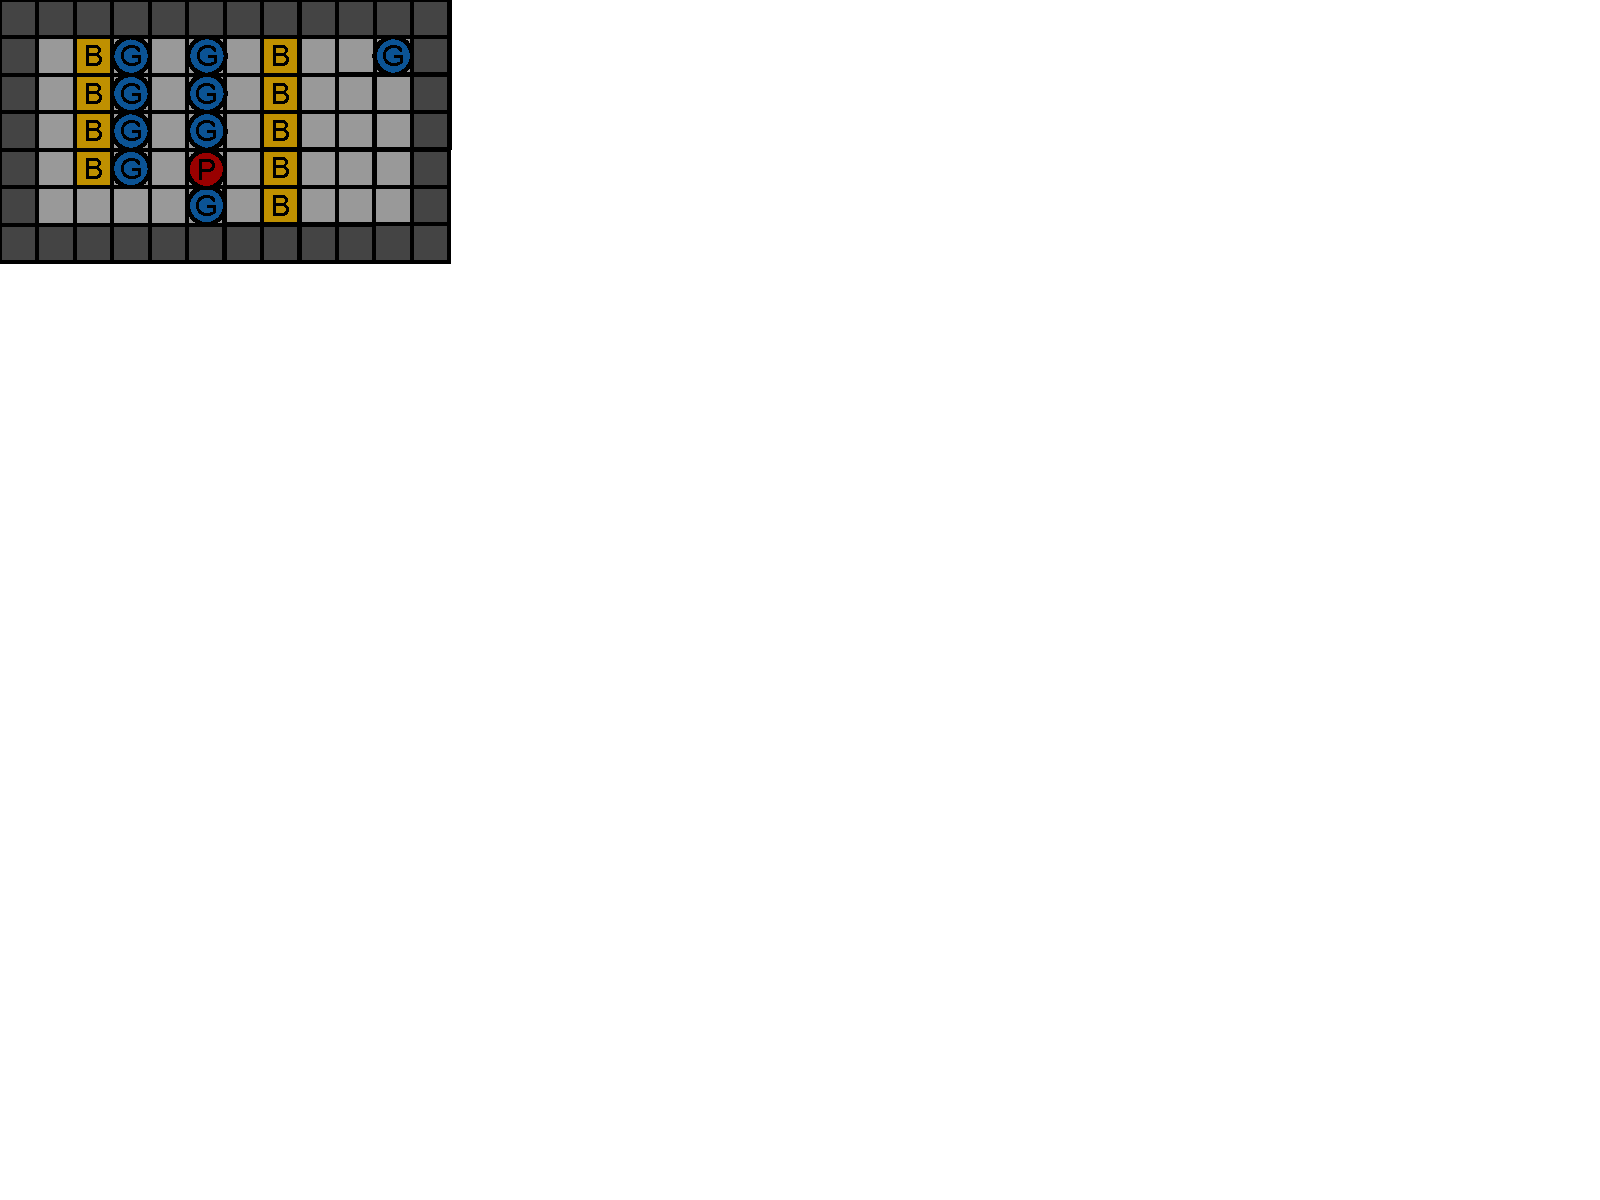
\includegraphics{figures/level136}
    \end{center}
    \caption{Example level illustrating the power of heuristics.}
    \label{fig:level136}
\end{figure}

To prune the tree is incredibly important, especially in the case with Sokoban,
as the search tree is incredibly large. We noticed large improvements when we
implemented the deadlock detection because of this very reason, it reduced the
size of the search tree. Similarly, the better performance of IDSPuller over
IDSPusher on many boards can be attributed to the built-in deadlock avoiding of
this algorithm.

We tried common code optimization techniques, such as pre-allocating objects and
re-using calculated values. Most of these optimizations did not yield any
substantial benefits. For instance when we optimized the most frequently called
function by inlining a function call and re-using a value,
updateReachabilityDFS, we achieved about 2-3 \% better.

% TODO: better what? faster solutions? more solved boards..?

Normal bugs is bound to arise in the development of any project. We had
particular problem with a couple of them which took us days to find and resolve.
The reason they are so hard to find is because of the incredibly large search
tree of Sokoban, it is simply to much information to go through in order to see
where the solver does something wrong. In those cases it is helpful to be able
to find and use a small level were the bug or performance issue shows itself.
Even though we were able to resolve all bugs eventually, we found the
bidirectional search particularly helpful when we had them as one solver could
compensate for the other ones bugs.


\section{Further improvements}

\subsection{A* and search heuristics}

A normal improvement to a Sokoban solver is to implement a heuristic. This is
usually done by implementing A* search, which is basically a normal search but
with a priority queue where the priority of the elements in the queue is
dictated by a heuristic. For example a good heuristic might be to prioritize
boards where many of the boxes are already on goal squares. In order for a
solver based on the A* algorithm to work well, it must not only use a good
heuristic that works for many different boards, but it also has to handle the
large amount of states that will be expanded.


\subsection{Corrals}

Corrals resembles no influence pushes in that moving a box inside a corral does
not affect the rest of the board.  There are several types of corrals. The
I-Corral (Figure~\ref{fig:corralsI}) is a corral where the player can push only
the outer boxes of the corral inwards, meanwhile an IP-Corral
(Figure~\ref{fig:corralsIP}) is an I-corral where you can move all of the outer
boxes. As with no influence pushes a corral need to be resolved sooner or later,
if the boxes are not all on goal squares.  As the corrals need to be resolved it
is better to solve them right away in order to detect possible deadlocks, rather
than to expand other possibilities and later find out they do not work because
of the same deadlock.

%\begin{figure}[h!]
    %\begin{center}
        %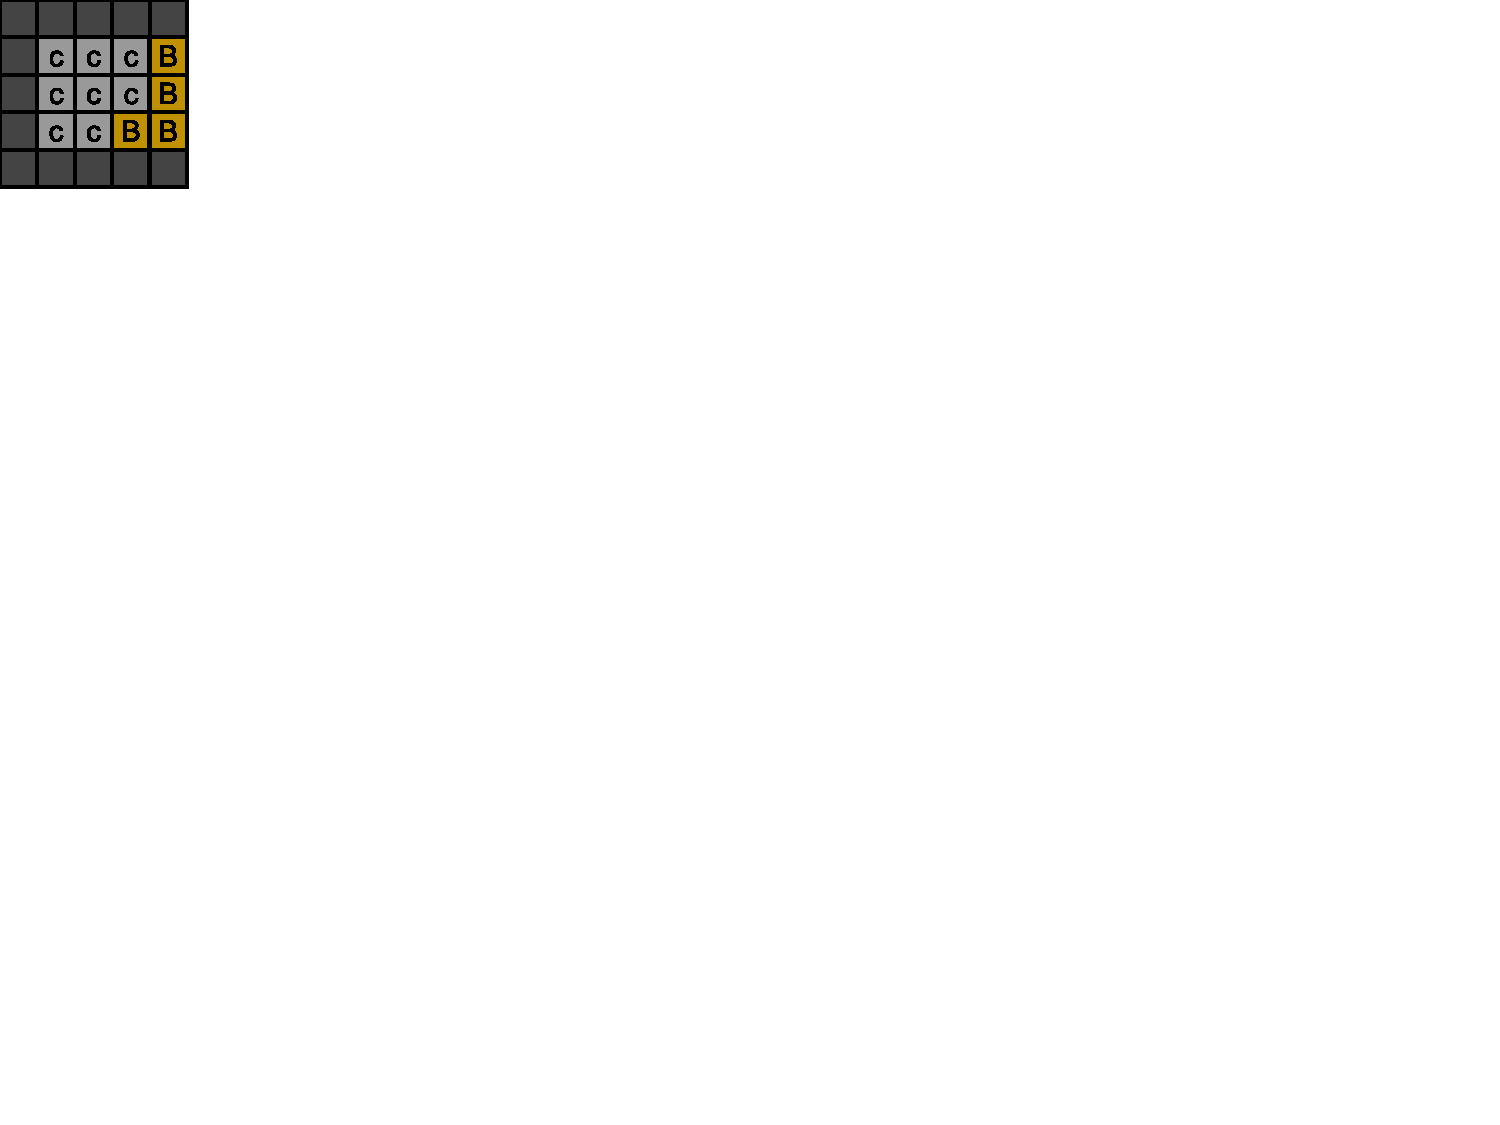
\includegraphics{figures/corralsI}
    %\end{center}
    %\caption{Example of I-corral.}
    %\label{fig:corralsI}
%\end{figure}

%\begin{figure}[h!]
    %\begin{center}
        %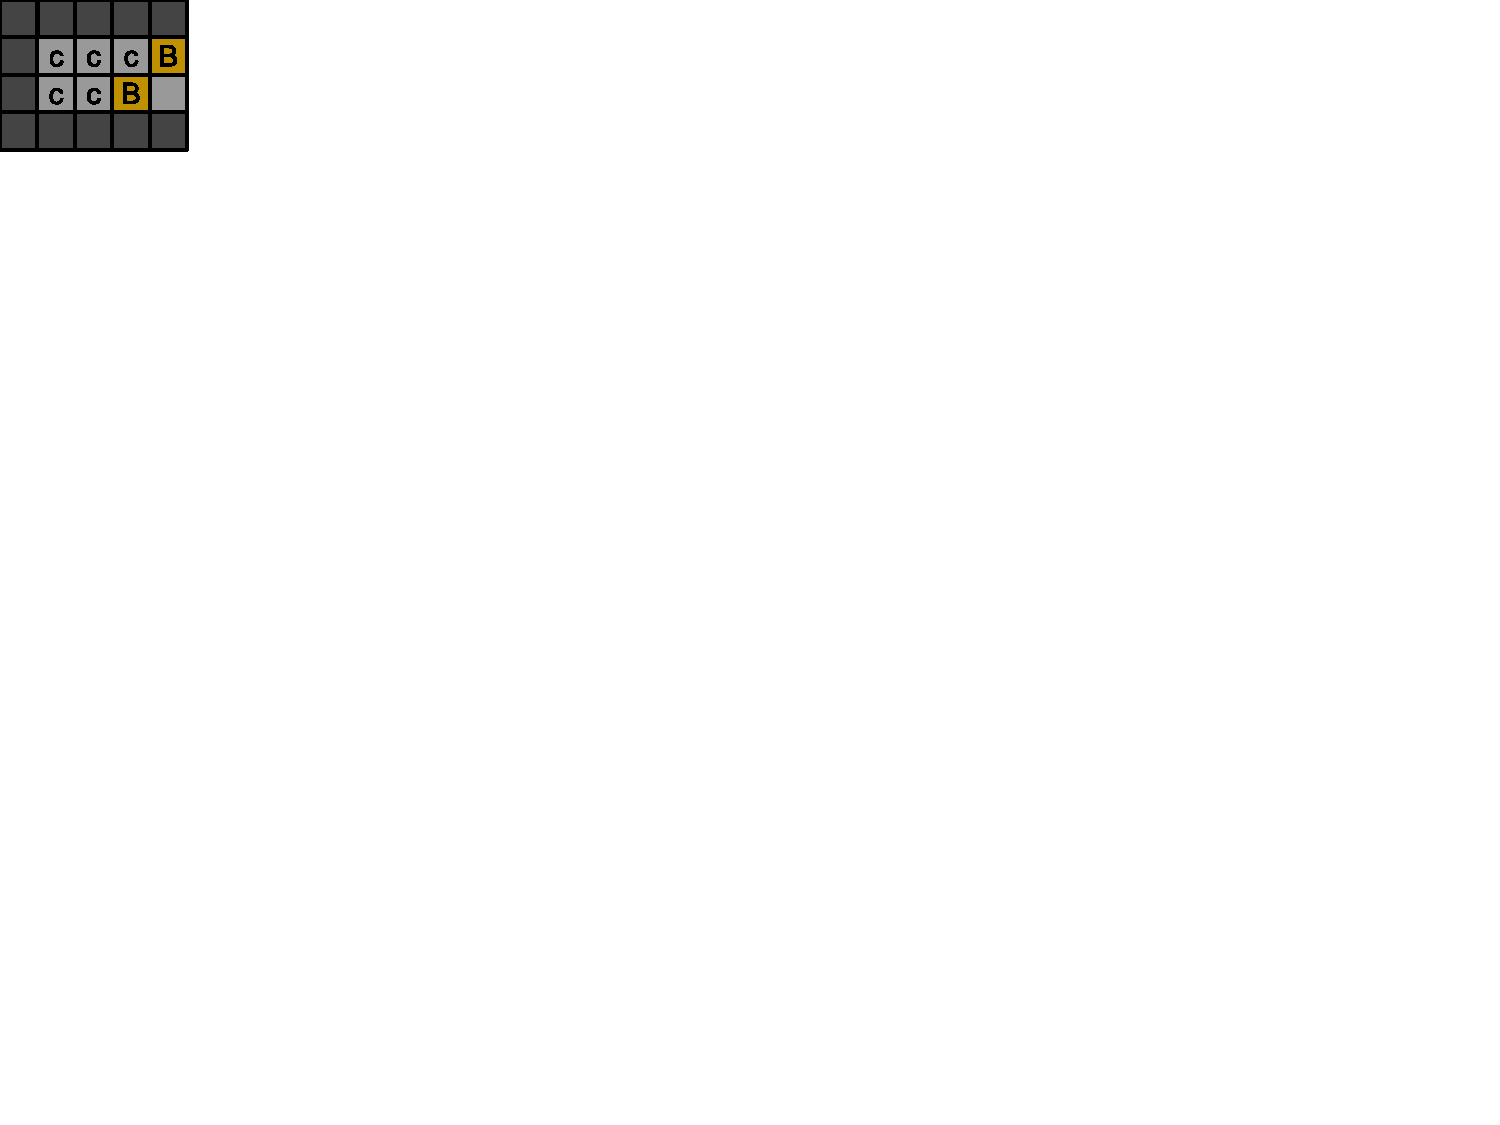
\includegraphics{figures/corralsIP}
    %\end{center}
    %\caption{Example of IP-corral.}
    %\label{fig:corralsIP}
%\end{figure}

\begin{figure}[h!]
  \begin{center}
    \subfigure[I-corral.]{\label{fig:corralsI}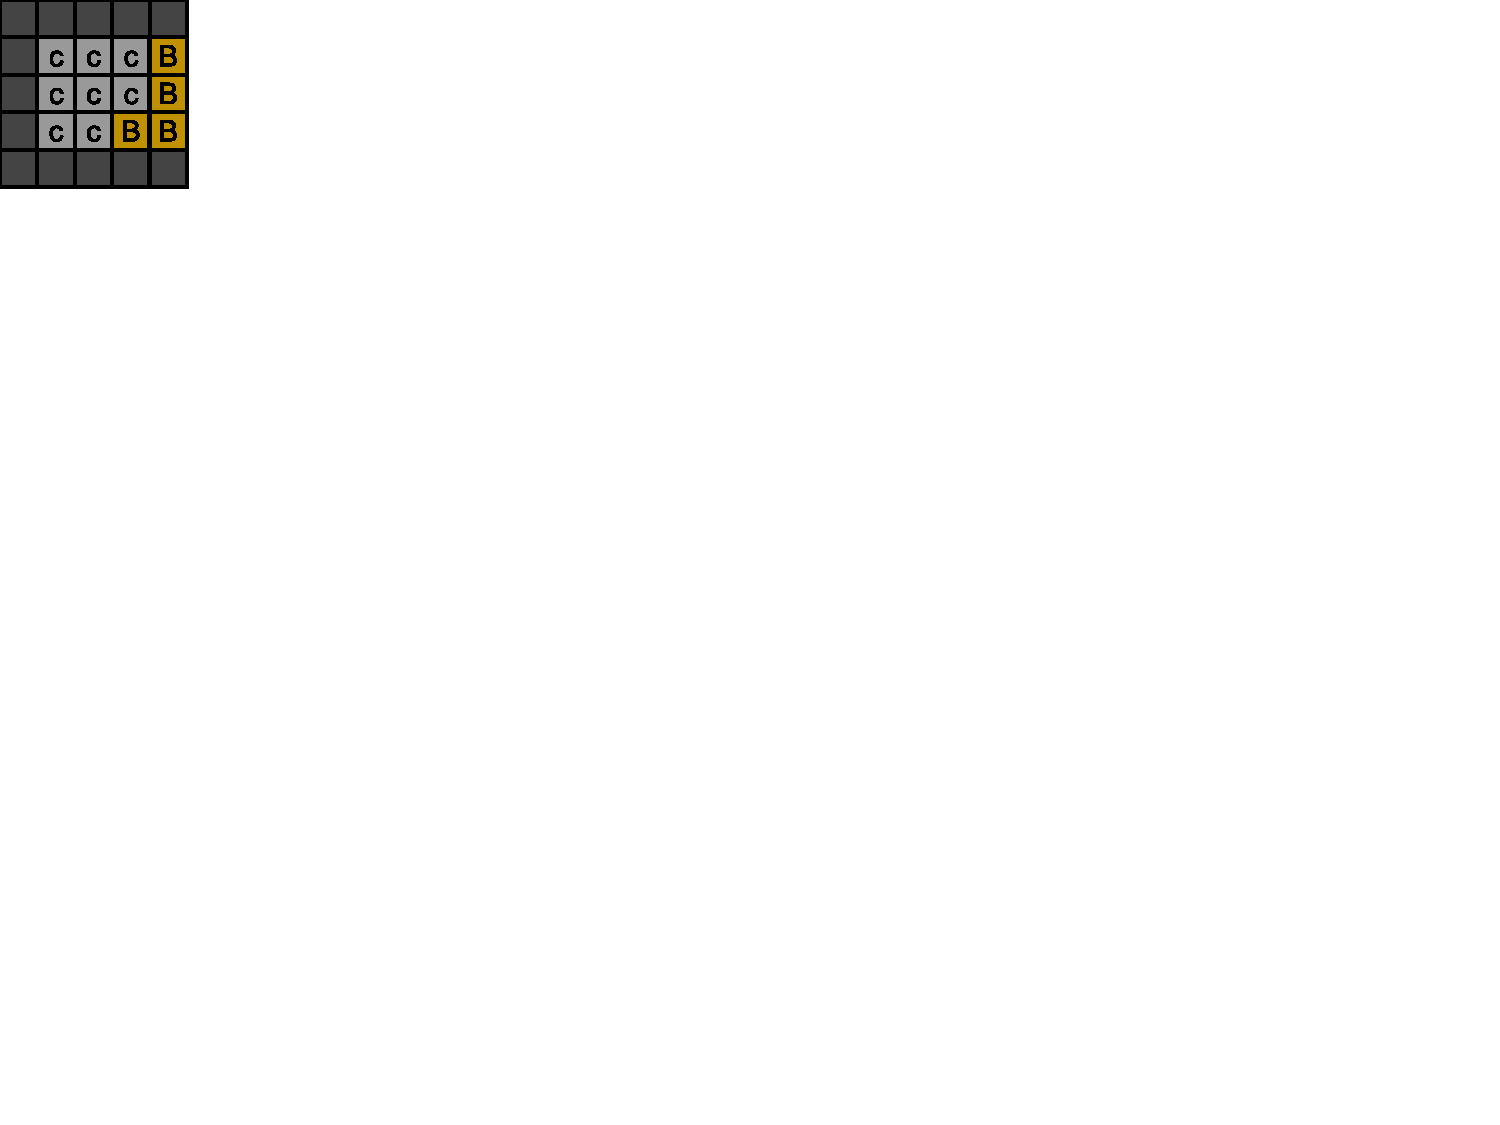
\includegraphics{figures/corralsI}}
    \subfigure[IP-corral.]{\label{fig:corralsIP}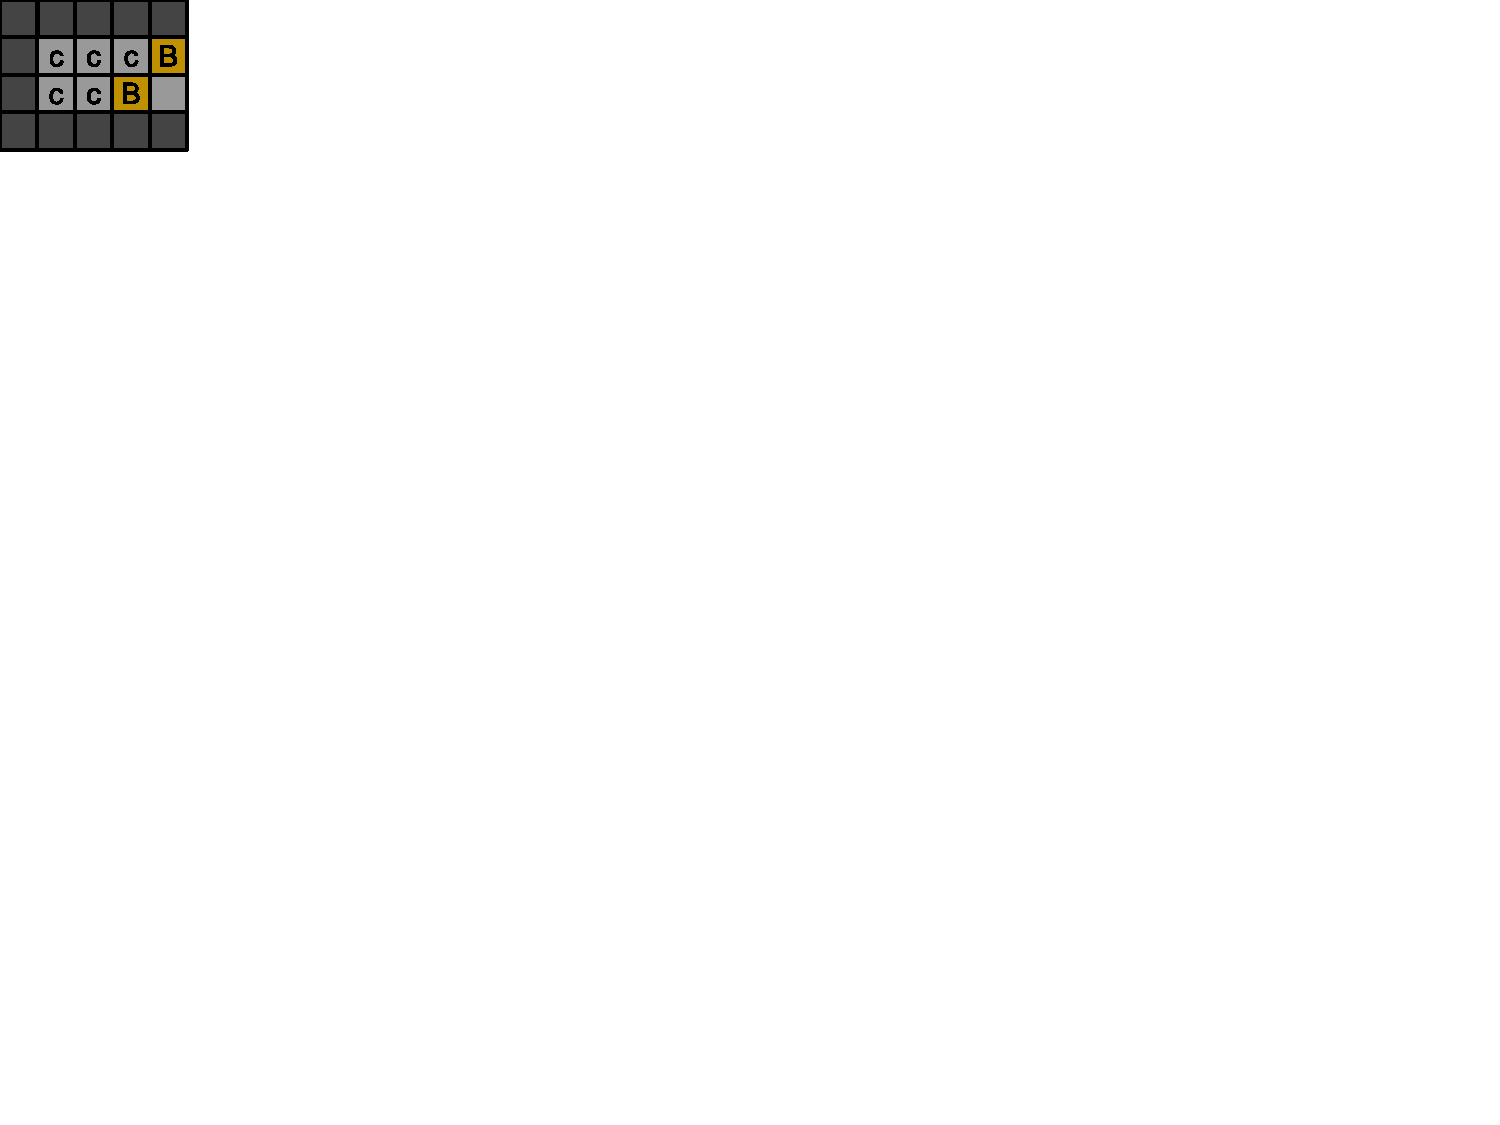
\includegraphics{figures/corralsIP}}
  \end{center}
  \caption{Examples of corrals.}
  \label{fig:corrals}
\end{figure}


\subsection{Incremental reachable square search}

A performance profiling of a non-trivial level shows that the function that
updates the reachable squares and boxes, updateReachabilityDFS, is the function
that executes for the largest amount of time. Typically it is between 30 to
70~\%, including garbage collection, for larger levels. But pushes often do not
change the reachable squares --- except the squares the box was pushed over ---
or only add more reachable squares. In such cases the array with reachable
squares does not have to be cleared and the search could be done incrementally,
that is, based on the existing data.


\part*{Conclusion}

%A few sentences that sums it all up

With relatively few and simple algorithms we have managed to implement a
working Sokoban solver with reasonable performance. Sadly there were some
algorithms which we did not have time to implement and we were not able to
solve all the levels we were given. However, it was meaningful to see what was
possible to do with mostly pruning techniques. The bidirectional solver was
particularly interesting because of the way it works and the incredibly large
performance improvement it gave us.


\bibliographystyle{plainnat}
\bibliography{references} 


\end{document}
